% Chapter 5: Results and Discussion
\label{chap:results}
This chapter presents the experimental results, comparing model performances across head, middle, and tail classes, and discusses the impact of different model architectures combined with different loss functions. First, the main findings are presented, followed by a detailed analysis of the results across experiments, and lastly a summary and discussion of the results. 

% \todo{Compare the different types of losses against each other. See \cite{menon2021longtaillearninglogitadjustment}.}

\section{Main Findings}
Across all models, Balanced Softmax Loss demonstrated the highest performance on tail classes for models trained on long-tailed datasets while maintaining consistent performance on head, middle, and overall long-tailed test sets. The highest top-1 accuracy for tail classes was achieved by the ResNet-50 architecture (Acc1: 60.53\%), closely followed by the ConvNeXt-Base architecture (Acc1: 57.89\%). However, this improved tail-class performance comes at the cost of head-class accuracy, where ConvNeXt-Base outperforms ResNet-50 with a top-1 accuracy of 86.85\% compared to 82.70\%. Overall, ConvNeXt-Base demonstrates better performance across all classes (Acc1: 82.30\%) on BS loss compared to ResNet-50 (Acc1: 79.16\%). See Tables \ref{tab:resnet_lt_acc1_1} and \ref{tab:conv_lt_acc1_1} for reference. 

Remarkably, SEQ Loss consistently underperformed when trained with ResNet-50, MobileNetV2, and ViT-B/16, but achieved comparably good results with ConvNeXt-Base on tail classes (Acc1: 47.37\%). Similarly, the ViT-B/16 architecture demonstrated the lowest overall accuracy when trained on both balanced and long-tailed datasets (Acc1: 59.06\%, see Table \ref{tab:vit_bal_acc1_1}), despite having the highest reported benchmark performance trained with balanced CIFAR-100 (Acc1: 93.95 \%) among all model architectures investigated in this thesis. This discrepancy suggests that the ViT-B/16 configuration used for the experiments in this thesis may not be well-suited for smaller-scale datasets such as CIFAR-100 without careful optimization as discussed in sections \ref{sec:ViTs} and \ref{sec:model_selection}.

\section{Overall Results}
This section presents the overall results of all experiments conducted in this thesis, highlighting the best and worst performance of each loss design on specific models without directly comparing losses or models. All models are first trained on a balanced CIFAR-100 dataset, to provide a reference point for evaluating the effectiveness of class re-balancing strategies. It provides an overview of all findings to understand how each combination of architecture and loss function behaves, starting with the ResNet-50 architecture.

\subsection{ResNet-50}

From Table \ref{tab:resnet_bal_acc1_1}, Softmax and Weighted Softmax yield identical performance when trained on balanced data due to their cross-entropy term in equations \eqref{eq:cb_loss} and \eqref{eq:wce_loss}. Balanced Softmax Loss demonstrates strong performance on the long-tailed test set (Acc1: 84.30\%) and head classes (Acc1: 84.60\%), while still performing comparably on tail classes. Notably, Sofmax Loss, Weighted Softmax Loss, and CB Loss all achieve top-1 accuracy of 94.74 \% on tail classes as the greates performance of all loss designs. Overall, the performance of the class re-balancing methods compare to that of the softmax baseline. The best performing loss design (softmax) perform with an accuracy of 83.24\%, not far behind the best published result for ResNet-50 with an accuracy of 86.90\% as seen in table \ref{tab:benchmark_comparison}.

\begin{table}[h!]
    \centering
    \caption{Evaluation results for ResNet50 trained on the custom balanced dataset, showing Acc1.}
    \begin{tabular}{cccccc}
        \toprule
        Loss Function & Balanced & Long-tailed & Head & Middle & Tail \\ 
        \midrule
        Softmax loss   & \textbf{0.8324}  & 0.8421 & 0.8448 & 0.8047 & \textbf{0.9474} \\
        Focal loss   & 0.8310  & 0.8344 & 0.8341 & \textbf{0.8166} & 0.9211 \\
        Weighted Softmax loss   & \textbf{0.8324} & 0.8421 & 0.8448 & 0.8047 & \textbf{0.9474} \\
        Class-balanced loss   &  0.8144 & 0.8173 & 0.8199 & 0.7751 & \textbf{0.9474} \\
        Balanced Softmax loss   & 0.8310 & \textbf{0.8430} & \textbf{0.8460} & 0.8107 & 0.9211 \\
        Equalization loss   & 0.8316 & 0.8354 & 0.8365 & \textbf{0.8166} & 0.8947 \\
        LDAM loss   & 0.7990 & 0.7983 & 0.8069 & 0.7337 & 0.8947 \\
        \bottomrule
    \end{tabular}
    \label{tab:resnet_bal_acc1_1}
\end{table}

From Table \ref{tab:resnet_lt_acc1_1}, Balanced Softmax Loss significantly improves tail-class accuracy (Acc1: 60.53\%), outperforming other loss designs, while also outperforming on balanced and middle sets. Softmax Loss achieves the best performance on the long-tailed dataset and head classes, indicating that while Balanced Softmax improves minority-class accuracy, Softmax remains strong for majority classes. Comparing with the results form table \ref{tab:resnet_bal_acc1_1}, most losses exhibits strong performance on head classes, except for SEQL with and underwhelming performance across all categories. Likewise, LDAM struggles with most categories, and particularly with tail classes.

\begin{table}[h!]
    \centering
    \caption{Evaluation results for ResNet50 trained on the long-tailed dataset, showing Acc1.}
    \begin{tabular}{cccccc}
        \toprule
        Loss Function & Balanced & Long-tailed & Head & Middle & Tail \\ 
        \midrule
        Softmax loss   & 0.5522 & \textbf{0.7954} & \textbf{0.8531} & 0.6391 & 0.2105 \\
        Focal loss   & 0.5456 & 0.7935 & 0.8483 & 0.6272 & 0.3158 \\
        Weighted Softmax loss   & 0.4976 & 0.7336 & 0.7915 & 0.5562 & 0.2368 \\
        Class-balanced loss   & 0.4970 & 0.7450 & 0.8069 & 0.5562 & 0.2105 \\
        Balanced Softmax loss   & \textbf{0.5908} & 0.7916 & 0.8270 & \textbf{0.6568} & \textbf{0.6053} \\
        Equalization loss   & 0.0886 & 0.1399 & 0.1505 & 0.1124 &  0.0263 \\
        LDAM loss   & 0.3742 & 0.5937 & 0.6469 & 0.4438 & 0.0789 \\
        \bottomrule
    \end{tabular}
    \label{tab:resnet_lt_acc1_1}
\end{table}


\subsection{MobileNetV2}

\begin{table}[H]
    \centering
    \caption{Top-1 accuracy results for MobileNetV2 on the balanced dataset across all loss functions.}
    \begin{tabular}{cccccc}
        \toprule
        Loss Function & Balanced & Long-tailed & Head & Middle & Tail \\ 
        \midrule
        Softmax   & 0.7978   & \textbf{0.8059} & \textbf{0.8069} & \textbf{0.7870} & 0.8684 \\
        Focal loss   & 0.8014   & 0.8011 & 0.7998 & \textbf{0.7870} & 0.8947 \\
        Weighted Softmax loss   & 0.7978   & \textbf{0.8059} & \textbf{0.8069} & \textbf{0.7870} & 0.8684 \\
        Class-balanced loss   & 0.8008   & 0.8049 & 0.8140 & 0.7456 & 0.8684 \\
        Balanced Softmax loss   & 0.8034  & 0.8030 & \textbf{0.8069} & 0.7574 & \textbf{0.9211} \\
        Equalization loss   &  \textbf{0.8078}  & 0.7916 & 0.7962 & 0.7396 & \textbf{0.9211} \\
        LDAM loss   &  0.7828   & 0.7821 & 0.7808 & 0.7574 & \textbf{0.9211} \\
        \bottomrule
    \end{tabular}
    \label{tab:mobilenet_bal_acc1_1}
\end{table}

As shown in Table \ref{tab:mobilenet_bal_acc1_1}, SEQL achieves the highest accuracy on the balanced test dataset (Acc1: 80.78\%) and, along with BS Loss and LDAM Loss, yields the best performance on tail classes (Acc1: 92.11\%), despite differences in loss designs. Not surprisingly, Softmax Loss and Weighted Softmax Loss yield the same accuracies across all test datasets due to shared cross-entropy designs, becoming indistinguishable when trained on balanced data, per equations \eqref{eq:ce_loss} and \eqref{eq:wce_loss}. Overall, all methods achieve results comparable to the softmax baseline and surpass the best published performance for MobileNetV2 trained on CIFAR-100, as shown in Table \ref{tab:benchmark_comparison}.

\begin{table}[h!]
    \centering
    \caption{Top-1 accuracy results for MobileNetV2 on the long-tailed dataset across all loss functions.}
    \begin{tabular}{cccccc}
        \toprule
        Loss Function & Balanced & Long-tailed & Head & Middle & Tail \\ 
        \midrule
        Softmax   & 0.5282   & 0.7735 & 0.8341 & 0.5917 & 0.2368 \\
        Focal loss   & 0.5200   & \textbf{0.7745} & \textbf{0.8389} & 0.5917 & 0.1579 \\
        Weighted Softmax loss   & 0.5016   & 0.7231 & 0.7808 & 0.5503 & 0.2105 \\
        Class-balanced loss   &  0.5034  & 0.7336 & 0.7938 & 0.5385 & 0.2632 \\
        Balanced Softmax loss   & \textbf{0.5796}   & 0.7650 & 0.8069 & \textbf{0.6331} & \textbf{0.4211} \\
        Equalization loss   &   0.0618 & 0.0647 & 0.0675 & 0.0592 & 0.0263 \\
        LDAM loss   & 0.4264 & 0.5899 & 0.6137 & 0.5444 & 0.2632 \\
        \bottomrule
    \end{tabular}
    \label{tab:mobilenet_lt_acc1_1}
\end{table}

From Table \ref{tab:mobilenet_lt_acc1_1}, Balanced Softmax Loss outperforms other losses in terms of balanced test accuracy (Acc1: 57.96\%) and especially tail classes (Acc1: 42.11\%). Although Softmax and Focal Loss surpass Balanced Softmax on the long-tailed dataset and head classes, the improvements Balanced Softmax provides for tail and middle classes are notable. SEQL shows an overwhelming underperformance compared with the balanced training in table \ref{tab:mobilenet_bal_acc1_1}, and now appears severely limited. The difference in performance on tail classes compared to the softmax baseline shows that loss functions designed for imbalance can provide more nuanced performance gains.


\subsection{ViT-B/16}

From Table \ref{tab:vit_bal_acc1_1}, LDAM Loss achieves the overall best performance for ViT-B/16 trained on balanced data. However, the overall performance remain far below the benchmark results for Vision Transformers on CIFAR-100, as seen in table \ref{tab:benchmark_comparison}. Although ViTs has achieved state-of-the-art performance in image classification, their architecture differs from CNNs, as described in section \ref{sec:ViTs}, and may require careful fine-tuning for optimal results. 

\begin{table}[h!]
    \centering
    \caption{Evaluation results for ViT-B/16 trained on the custom balanced dataset, showing Acc1.}
    \begin{tabular}{cccccc}
        \toprule
        Loss Function & Balanced & Long-tailed & Head & Middle & Tail \\ 
        \midrule
        Softmax loss   & 0.5620 & 0.5671 & 0.5521 & 0.6036 & 0.7368 \\
        Focal loss   & 0.5516 & 0.5538 & 0.5438 & 0.5680 & 0.7105 \\
        Weighted Softmax loss   & 0.5620 & 0.5671 & 0.5521 & 0.6036 & 0.7368 \\
        Class-balanced loss   & 0.5432 & 0.5452 & 0.5427 & 0.5207 & 0.7105 \\
        Balanced Softmax loss   & 0.5628 & 0.5642 & 0.5640 & 0.5325 & 0.7105 \\
        Equalization loss   & 0.5582 & 0.5547 & 0.5462 & 0.5680 & 0.6842 \\
        LDAM loss   & \textbf{0.5906} &  \textbf{0.6013} & \textbf{0.5924} & \textbf{0.6095} & \textbf{0.7632} \\
        \bottomrule
    \end{tabular}
    \label{tab:vit_bal_acc1_1}
\end{table}


\begin{table}[h!]
    \centering
    \caption{Evaluation results for ViT-B/16 trained on the long-tailed dataset, showing Acc1.}
    \begin{tabular}{cccccc}
        \toprule
        Loss Function & Balanced & Long-tailed & Head & Middle & Tail \\ 
        \midrule
        Softmax loss   & 0.2254 & \textbf{0.4367} & \textbf{0.5071} & 0.1775 & 0.0263 \\
        Focal loss   & 0.2210 & 0.4206 & 0.4834 & 0.1953 & 0.0263 \\
        Weighted Softmax loss   & 0.1284 & 0.1760 & 0.1919 & 0.1302 & 0.0263 \\
        Class-balanced loss   & 0.1346 & 0.1865 & 0.2014 & 0.1361 & 0.0789 \\
        Balanced Softmax loss   & \textbf{0.2460} & 0.4244 & 0.4822 &  \textbf{0.2130} & 0.0789 \\
        Equalization loss   & 0.1686 & 0.2778 & 0.3140 & 0.1361 & \textbf{0.1053} \\
        LDAM loss   & 0.1570 & 0.2750 & 0.3140 & 0.1361 & 0.0263 \\
        \bottomrule
    \end{tabular}
    \label{tab:vit_lt_acc1}
\end{table}

The results from Table \ref{tab:vit_lt_acc1} show low performance across all loss designs. Balanced Softmax Loss slightly improves results on balanced and middle categories, while Softmax Loss achieves the highest accuracy on the long-tailed dataset and head classes. The best performance on tail classes (Acc1: 10.53\%) is achieved by SEQL, however, still unsatisfactory. This pattern suggests that the ViT-B/16 architecture may not be sufficient for robust performance on smaller-scale, long-tailed datasets and may require furhter adjustments in the training pipeline, as outlined in section \ref{sec:ViTs}. 

\subsection{ConvNeXt Base}
From Table \ref{tab:conv_bal_acc1_1}, CB Loss achieves the highest balanced test accuracy of 83.64\% while the Softmax Loss, Weighted Softmax loss, and BS loss tie for top performance on the long-tailed dataset (Acc1: 94.74\%). Softmax Loss and weighted softmax loss yield same perfomance across all categories du to their shared design on balanced datasets. The saturation of tail-class performance is likely due to the quality or quantity of tail classes. For comparison, the best published result for a ConvNext architecture trained with CIFAR-100 achieve an accuarcy of 94.04\% (see table \ref{tab:benchmark_comparison}), the best perfomance of on the balanced test set is in alignment yields an accuracy of 83.98\%, implying room for improvement in the training pipeline.

\begin{table}[h!]
    \centering
    \caption{Evaluation results for ConvNeXt Base trained on the custom balanced dataset, showing Acc1.}
    \begin{tabular}{cccccc}
        \toprule
        Loss Function & Balanced & Long-tailed & Head & Middle & Tail \\ 
        \midrule
        Softmax loss   & 0.8332 & \textbf{0.8535} & \textbf{0.8566} & 0.8166 & \textbf{0.9474} \\
        Focal loss   & 0.8314 & 0.8487 & 0.8507 & \textbf{0.8284} & 0.8947 \\
        Weighted Softmax loss   & 0.8332 & \textbf{0.8535} & \textbf{0.8566} &  0.8166 & \textbf{0.9474} \\
        Class-balanced loss   & \textbf{0.8398} & 0.8344 & 0.8389 & 0.7929 & 0.9211 \\
        Balanced Softmax loss   & 0.8364 & 0.8344 & 0.8365 & 0.7988 & \textbf{0.9474} \\
        Equalization loss   & 0.8322 & 0.8392 & 0.8412 & 0.8107 & 0.9211 \\
        LDAM loss   & 0.8316 & 0.8373 & 0.8412 & 0.8047 & 0.8947 \\
        \bottomrule
    \end{tabular}
    \label{tab:conv_bal_acc1_1}
\end{table}


\begin{table}[h!]
    \centering
    \caption{Evaluation results for ConvNeXt Basetrained on the long-tailed dataset, showing Acc1.}
    \begin{tabular}{cccccc}
        \toprule
        Loss Function & Balanced & Long-tailed & Head & Middle & Tail \\ 
        \midrule
        Softmax loss   & 0.5972 & \textbf{0.8316} & \textbf{0.8898} & \textbf{0.6568} & 0.3158 \\
        Focal loss   & 0.5938 & 0.8145 & 0.8685 & \textbf{0.6568} & 0.3158 \\
        Weighted Softmax loss   & 0.4090 & 0.6356 & 0.6848 & 0.4911 & 0.1842 \\
        Class-balanced loss   & 0.3436 & 0.5756 & 0.6469 & 0.3254 & 0.1053 \\
        Balanced Softmax loss   & \textbf{0.6460} & 0.8230 & 0.8685 & 0.6509 & \textbf{0.5789} \\
        Equalization loss   & 0.5948 & 0.7973 & 0.8460 & 0.6272 & 0.4737 \\
        LDAM loss   & 0.3770 & 0.5956 & 0.6445 & 0.4260 & 0.2632 \\
        \bottomrule
    \end{tabular}
    \label{tab:conv_lt_acc1_1}
\end{table}

Table \ref{tab:conv_lt_acc1_1} shows that Balanced Softmax Loss significantly outperforms other methods on the balanced test set (Acc1: 64.60\%) and tail classes (Acc1: 57.89\%). Softmax achieves the best performance on the long-tailed dataset, as well as on head and middle classes. Notably, SEQL delivers comparable results across all categories, in contrast to its performance with other model architectures, where it fell short compared to other loss designs.

\section{Benchmarks}
Table \ref{tab:benchmark_comparison} compares the best results from the models trained on the balanced CIFAR-100 dataset in this thesis with published benchmarks using the same backbone architectures. This comparison serves as a reference to ensure the results align with expectations and to identify any potential discrepancies. 

For MobileNetV2, the results in this thesis surpass the published benchmarks. This could be attributed to improved loss function designs. On the other hand, both ResNet-50 and ConvNeXt-Base exhibits lower accuracies compared to benchmarks, which may be explained by differences in training pipelines.

The most significant deviation is observed with ViT-B/16, where the accuracy falls far short of the benchmark. This discrepancy suggests that the configuration for ViT-B/16 may not optimized for training with small-scale datasets, as outlined in section \ref{sec:ViTs}. 

Overall, these results indicate that the experimental setup is effective for most models but highlights potential limitations for transformer-based architectures such as ViT-B/16. Future investigation could lead to and understanding of these discrepancies.

\begin{table}[H]
    \centering
    \caption{Comparison of model performance on balanced CIFAR-100 with published benchmarks.}
    \begin{tabular}{|l|c|c|}
    \hline
    \textbf{Model}        & \textbf{Result (Acc1)} & \textbf{Benchmark Result (Acc1)}  \\ \hline
    MobileNetV2           & 80.78\%               & 73.20\% \cite{park2022bitatneuralnetworkbinarization}  \\ \hline
    ResNet50            & 83.24\%               & 86.90\% \cite{wightman2021resnetstrikesbackimproved}  \\ \hline
    ViT-B/16              & 59.06\%               & 93.51\% \cite{ye2023partialfinetuningsuccessorfinetuning} \\ \hline
    ConvNeXt Base         & 83.98\%               & 94.04\% \cite{ye2023partialfinetuningsuccessorfinetuning}  \\ \hline
    \end{tabular}
    \label{tab:benchmark_comparison}
\end{table}



\section{Performance Comparisons}
\subsection{Model Performance}
The models are evaluated based on the mean and standard deviation of their results across all loss functions. These statistics are visualized in Figure \ref{fig:mean_loss_comparison} and detailed in Table \ref{tab:model_performance_summary}. Here, the performances of the models MobileNetV2, ResNet-50, ViT-B/16, and ConvNeXt-Base are shown across the evaluation categories: Balanced, Long-Tailed, Head, Middle, and Tail. Each model is slightly offset along the x-axis to avoid overlap. Each point represents the mean accuracy of a model for a specific category and the bars represent the standard deviation. The error bars indicate the variability in accuracy across different loss functions for each model and category. A longer error bar demonstrate a less consistent performance, dependent on the chosen loss function, while shorter error bars indicate consistant performance adhering to the specific model.

Ignoring the sub-par performance of the ViT-B/16 architecture, the shorter errorbars for ConvNeXt-Base in figure \ref{fig:mean_loss_comparison} indicate that its architecture may be more robust to class-sensitive strategies than other architechtures. Additionally, this architecture displays the greatest mean accuracies across all categories. Contrary, the performance of MobileNetV2 shows a greater sensitivity to the choice of loss design with the exception of ResNet-50 on tail classes. ViT-B/16 shows a consistently lower mean accuracy, indicating that transformer-based approaches may require additional adaptations for smaller-scale or imbalanced datasets, as discussed in \ref{sec:model_selection}. Overall, ConvNeXt-Base maintains strong and stable performance across all categories, benefiting from Balanced Softmax Loss as seen in table \ref{tab:conv_lt_acc1_1}.

\begin{figure}[h!]
    \centering
    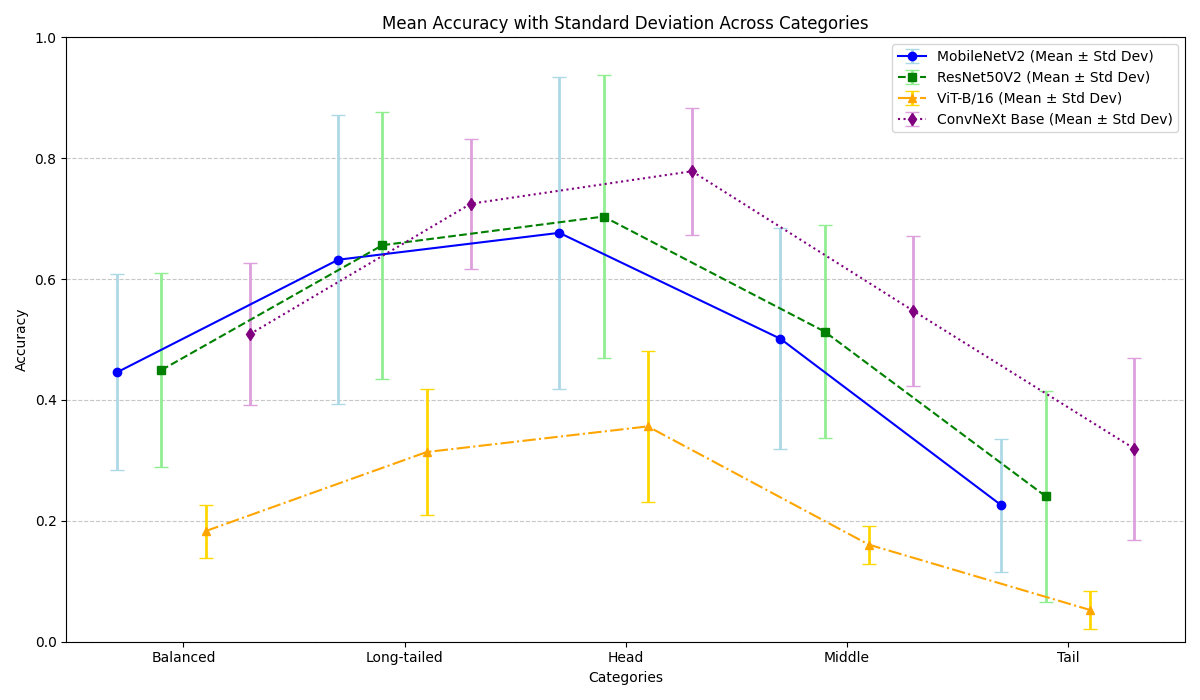
\includegraphics[width=0.9\textwidth]{Images/Plots/mean_loss_comparison.png}
    \caption{Mean Accuracy with Standard Deviation Across Categories for MobileNetV2, ResNet-50, ViT-B/16, and ConvNeXt Base trained with CIFAR-100-LT.}
    \label{fig:mean_loss_comparison}
\end{figure}

\begin{table}[h!]
    \centering
    \caption{Performance Summary Across Categories (Mean ± Std)}
    \scriptsize
    \begin{tabular}{lccccc}
        \toprule
        Model & Balanced & Long-tailed & Head & Middle & Tail \\
        \midrule
        MobileNetV2 
        & 0.4459 ± 0.1623 & 0.6320 ± 0.2391 & 0.6765 ± 0.2585 & 0.5013 ± 0.1832 & 0.2256 ± 0.1107 \\
        ResNet-50 
        & 0.4494 ± 0.1605 & 0.6561 ± 0.2207 & 0.7035 ± 0.2348 & 0.5131 ± 0.1767 & 0.2406 ± 0.1743 \\
        ViT-B/16 
        & 0.1830 ± 0.0438 & 0.3139 ± 0.1047 & 0.3563 ± 0.1250 & 0.1606 ± 0.0315 & 0.0526 ± 0.0315 \\
        ConvNeXt-Base 
        & 0.5088 ± 0.1170 & 0.7247 ± 0.1077 & 0.7784 ± 0.1050 & 0.5477 ± 0.1243 & 0.3196 ± 0.1505 \\
        \bottomrule
    \end{tabular}
    \label{tab:model_performance_summary}
\end{table}

\subsection{Loss Comparison}
The Balanced Softmax Loss emerges as the overall best performing loss design across all models with the least variance in performance across test categories, excluding the performances of ViT-B/16, as figures \ref{fig:resnet_lt_loss_comparison}, \ref{fig:mobilenet_lt_loss_comparison}, and \ref{fig:conv_lt_loss_comparison} illustrate. For reference, the performance of ViT-B/16 is illustrated in figure \ref{fig:vit_lt_loss_comparison}. From figure \ref{fig:conv_lt_loss_comparison}, the SEQL stands out in performance across all categories, and nearly competes with BS loss in terms of variance. In contrast, SEQL exhibits the worst performance on both ResNet-50 and MobileNetV2 (see Figures \ref{fig:resnet_lt_loss_comparison} and \ref{fig:mobilenet_lt_loss_comparison}), possibly because these architectures are less robust to the large negative logits and masking strategy enforced by SEQL as opposed to ConvNeXt-Base.

These result are further underlined in figure \ref{fig:loss_comparison_bars}, where the mean and standard deviation of the loss functions across the four backbone architectures are illustrated. Here, the Balanced Softmax Loss shows a better average perfomance on tail classes, while also displaying the smoothest variation across evaluation categories, ignoring the SEQL. Additionally, the standard deviation suggests that the perfomance of the Balanced Softmax Loss on tail classes depend on the model architecture. Table \ref{tab:performance_summary} display the exact values of the mean and standard deviations shown in figure \ref{fig:loss_comparison_bars}. 


\begin{figure}[h!]
    \centering
    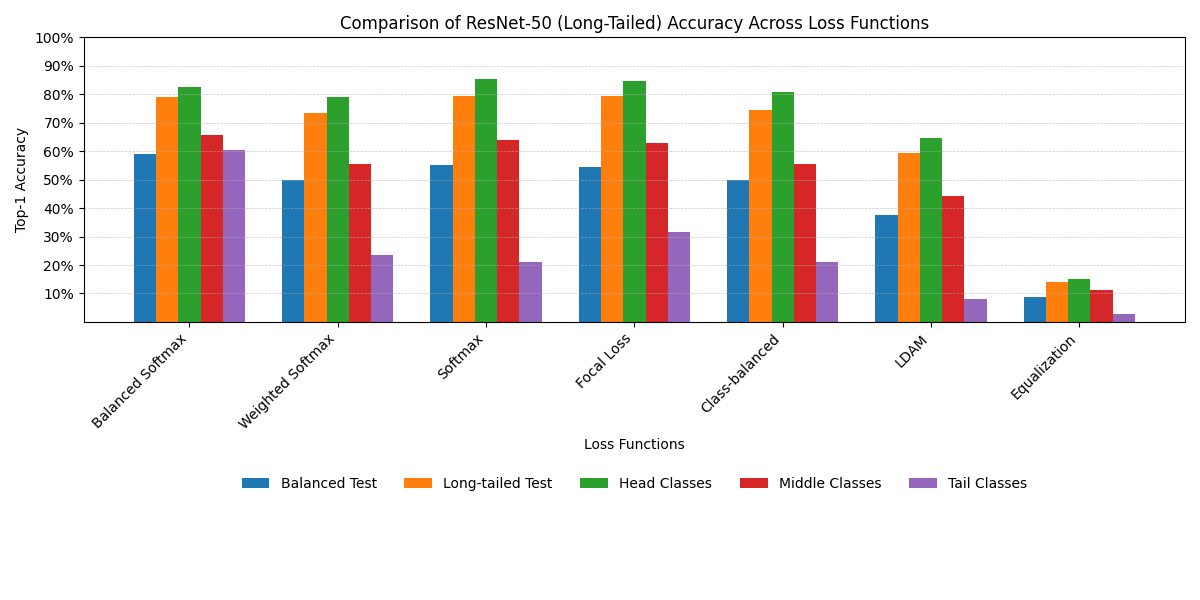
\includegraphics[width=0.9\textwidth]{Images/Plots/resnet_lt_loss_comparison.png}
    \caption{ResNet-50 top 1 accuracy across test categories (Balanced, Long-tailed, Head, Middle, Tail) for different loss functions.}
    \label{fig:resnet_lt_loss_comparison}
\end{figure}
\FloatBarrier

\begin{figure}[h!]
    \centering
    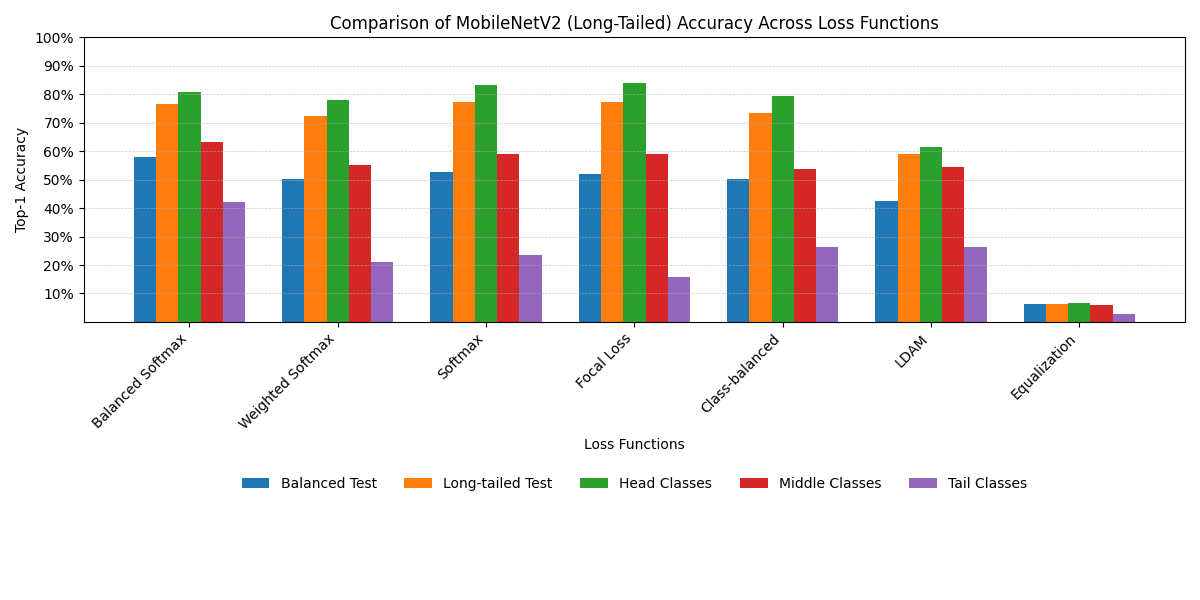
\includegraphics[width=0.9\textwidth]{Images/Plots/mobilenet_lt_loss_comparison.png}
    \caption{MobileNetV2 top 1 accuracy across test categories (Balanced, Long-tailed, Head, Middle, Tail) for different loss functions.}
    \label{fig:mobilenet_lt_loss_comparison}
\end{figure}
\FloatBarrier

\begin{figure}[h!]
    \centering
    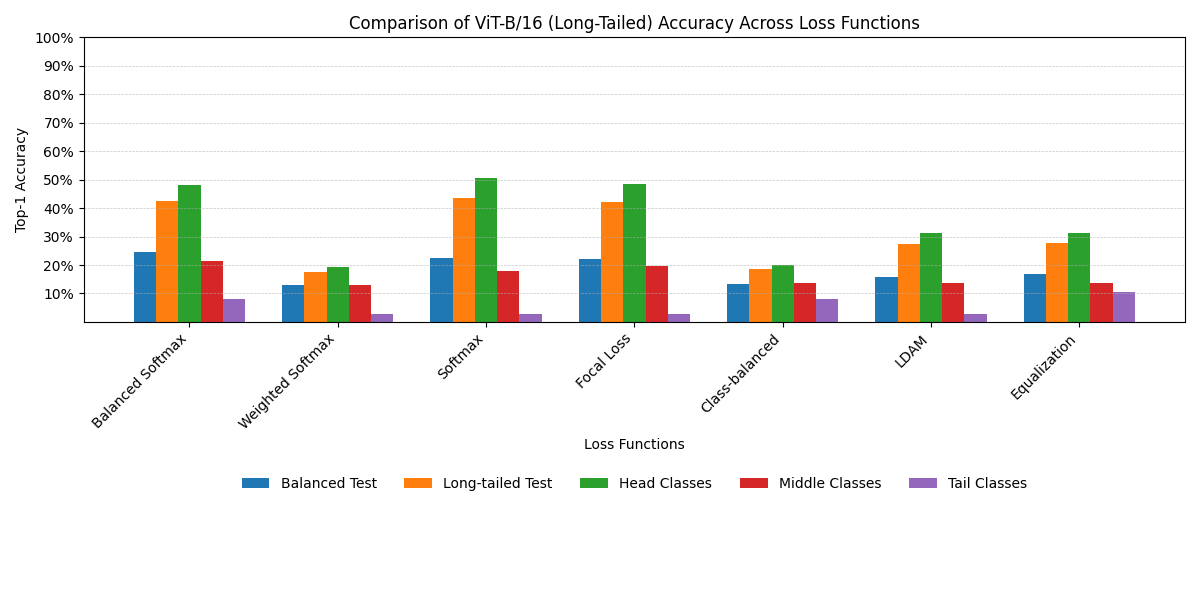
\includegraphics[width=0.9\textwidth]{Images/Plots/vit_lt_loss_comparison.png}
    \caption{ViT-B/16 top 1 accuracy across test categories (Balanced, Long-tailed, Head, Middle, Tail) for different loss functions.}
    \label{fig:vit_lt_loss_comparison}
\end{figure}
\FloatBarrier

\begin{figure}[h!]
    \centering
    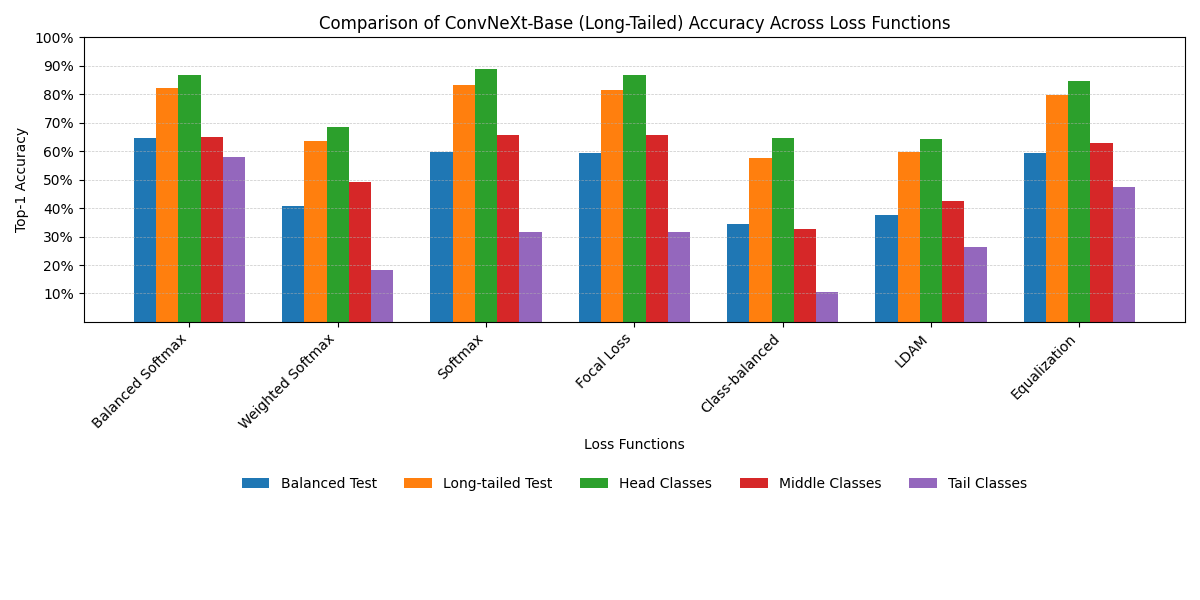
\includegraphics[width=0.9\textwidth]{Images/Plots/convnext_lt_loss_comparison.png}
    \caption{ConvNeXt-Base top 1 accuracy across test categories (Balanced, Long-tailed, Head, Middle, Tail) for different loss functions.}
    \label{fig:conv_lt_loss_comparison}
\end{figure}
\FloatBarrier


\begin{figure}[h!]
    \centering
    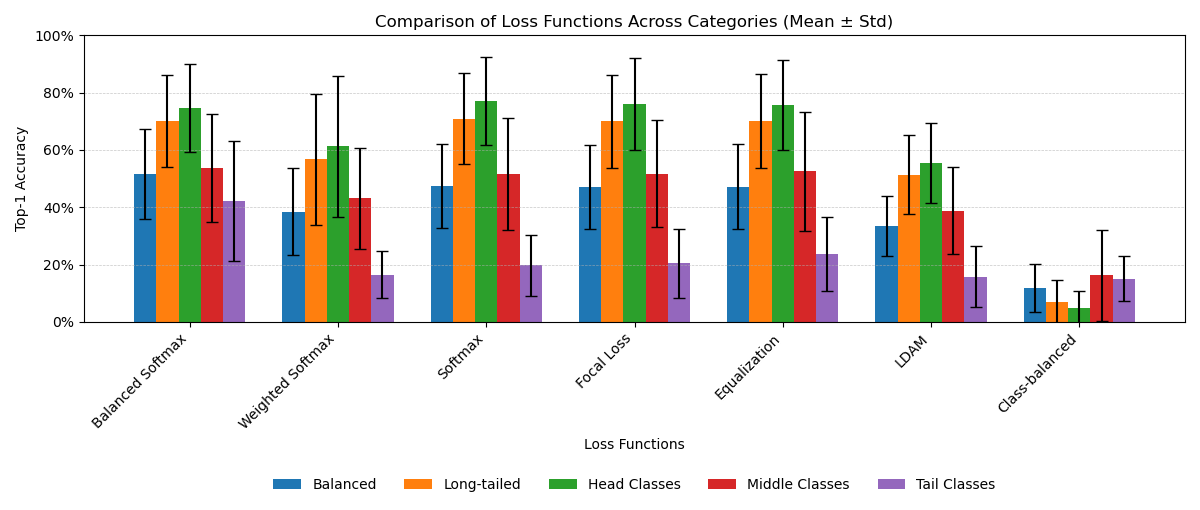
\includegraphics[width=0.9\textwidth]{Images/Plots/loss_function_bar_plot_mean_std.png}
    \caption{Performance trends of different loss functions across evaluation categories. Error bars indicate the standard deviation of accuracy across models, highlighting variability in performance for each loss function.}
    \label{fig:loss_comparison_bars}
\end{figure}
\FloatBarrier


\begin{table}[h!]
    \centering
    \caption{Performance Summary Across Categories (Mean ± Std)}
    \scriptsize
    \begin{tabular}{lccccc}
        \toprule
        Loss Function & Balanced & Long-tailed & Head & Middle & Tail \\
        \midrule
        Balanced Softmax 
        & $0.5156 \pm 0.1577$ & $0.7010 \pm 0.1610$ & $0.7462 \pm 0.1540$ & $0.5385 \pm 0.1881$ & $0.4211 \pm 0.2097$ \\
        Weighted Softmax 
        & $0.3842 \pm 0.1522$ & $0.5671 \pm 0.2290$ & $0.6123 \pm 0.2462$ & $0.4320 \pm 0.1761$ & $0.1645 \pm 0.0819$ \\
        Softmax 
        & $0.4758 \pm 0.1466$ & $0.7093 \pm 0.1587$ & $0.7710 \pm 0.1537$ & $0.5163 \pm 0.1970$ & $0.1974 \pm 0.1061$ \\
        Focal Loss 
        & $0.4701 \pm 0.1462$ & $0.7008 \pm 0.1624$ & $0.7598 \pm 0.1599$ & $0.5178 \pm 0.1876$ & $0.2039 \pm 0.1211$ \\
        Class-balanced 
        & $0.3697 \pm 0.1500$ & $0.5602 \pm 0.2259$ & $0.6123 \pm 0.2454$ & $0.3891 \pm 0.1720$ & $0.1645 \pm 0.0753$ \\
        LDAM 
        & $0.3337 \pm 0.1041$ & $0.5136 \pm 0.1377$ & $0.5548 \pm 0.1396$ & $0.3876 \pm 0.1520$ & $0.1579 \pm 0.1069$ \\
        Equalization 
        & $0.2285 \pm 0.2151$ & $0.3199 \pm 0.2860$ & $0.3445 \pm 0.3028$ & $0.2337 \pm 0.2289$ & $0.1579 \pm 0.1852$ \\
        \bottomrule
    \end{tabular}
    \label{tab:performance_summary}
\end{table}



\section{Summary and Discussion}
The overall best performance on tail classes was achieved by the Balanced Softmax Loss, which proved to be consistent across all models while also achieving competing results on other test categories. Furthermore, these findings highlight the impact of model architecture combined with loss designs, as the standard deviation demonstrates when comparing figures \ref{fig:mean_loss_comparison} and \ref{fig:loss_comparison_bars}. Here, the longer errorbars suggests the dependency of loss design and model architecture, respectively. Further investigation of model and loss design combinations could lead to greater tail-class performance.

Although the CB Loss' overall superior performance on tail classes, this performance accuracy often came with trade-offs in performance on head classes. For example, while ResNet-50 achieved the highest top 1 accuracy of 60.53\% on tail classes using Balanced Softmax, compared to that of ConvNeXt Base (Acc1: 57.89\%), head-class accuracy (82.70\%) lagged behind ConvNeXt Base (86.85\%). This trade-off highlights the challenge of optimizing for both head and tail classes simultaneously and indicates that Balanced Softmax prioritizes tail-class adjustments at the expense of head-class performance. 

SEQL, in contrast, consistently underperformed across all models and test categories with the exception of ConvNeXt-Base. This suggests that the down-weighting of the negative gradients posed by the SEQL affect the model's ability to distinguish classes from one another, as discussed in section \ref{sec:loss_selection}. The ConvNetxt architecture includes designs components that could help mitigate the performance drop imposed by the heavy masking, such as LayerNorm (see section \ref{sec:convnext}). When training on a small datasets like the long-tailed CIFAR-100, the use of SEQL could result in the model not receiving an adequate number of samples for training when negative gradients are down-weighted. Moreover, the model fails to learn fine-grained distinctions necessary to achieve high discriminative abilities.  

Likewise, the ViT-B/16 architecture underperformed significantly across all loss designs (including the softmax baseline), categories, and training datasets, with the best accuracy of 59.06\% on a balanced training dataset compared to its benchmark of 93.95\% \cite{ye2023partialfinetuningsuccessorfinetuning}. These results indicate that the default ViT-B/16 architecture may not be well-suited for long-tailed datasets without further optimization \cite{menon2021longtaillearninglogitadjustment,loshchilov2018fixing}. These could include a carefully chosen optimizer, longer training, or larger dataset \cite{beyer2022betterplainvitbaselines}. Comparatively, the CNN architectures displayed overall better performance with the same setup. 

The high and equal tail-class performances of ResNet-50, MobileNetV2, and ConvNeXt-Base trained on the balanced CIFAR-100 (see tables \ref{tab:resnet_bal_acc1_1}, \ref{tab:mobilenet_bal_acc1_1}, and \ref{tab:conv_bal_acc1_1}) suggests that tail-class performance may have reached a saturation point due to the limited number of samples in tail classes. These limitations could be investigated through testing on a larger datasets. 

\todo{Include discussion of the choice of adam optimizer over the SGD.}


The performance of the LDAM could potentially improve by including the deferred re-weighting scheme (DRW), also introduced by Cao et al. \cite{cao2019learningimbalanceddatasetslabeldistributionaware}. According to related work \cite{menon2021longtaillearninglogitadjustment}, the DRW significanlty improves performance on long-tailed datasets in contrast to relying solely on LDAM for effective class re-balancing. The authors of behind LDAM achieved top-1 error of 57.96\% on CIFAR-100-LT with imbalance ratio of 100 on ResNet-32 with LDAM-DRQ. The experiments in this thesis yielded \todo{make this}.

The decision to derive test data from the training set, rather than splitting the validation set to match the class distribution to that of the ImageNet-LT (see section \ref{sec:dataset_specs}), could also influence the results, since the training data would include more samples. Likewise, the performance of the combinations of model architectures and loss designs could benefit from training with a larger dataset, like ImageNet and ImageNet-LT. Furthermore, these larger long-tailed benchmarks follow the Pareto distribution rather than an exponential decay, mirroring a natural occuring long-tailed dataset, as discussed in sections \ref{sec:lt-datasets} and \ref{sec:dataset_specs}.  


Overall, these findings emphasize the importance of aligning loss functions with both dataset characteristics and model architectures to address the challenges of deep long-tailed learning. They also highlight the need for a nuanced approach that balances improvements in tail-class accuracy with minimal trade-offs in head-class and overall performance.

\todo{Adam optimization:}
Figure 1: Mean and standard deviation over 5 runs of per-class weight norms for a ResNet-32 under
momentum and Adam optimisers. We use long-tailed (“LT”) versions of CIFAR-10 and CIFAR-100,
and sort classes in descending order of frequency; the first class is 100 times more likely to appear
than the last class. Both optimisers yield solutions with comparable balanced error. However, the
weight norms have incompatible trends: under momentum, the norms are strongly correlated with
class frequency, while with Adam, the norms are anti-correlated or independent of the class frequency.
Consequently, weight normalisation under Adam is ineffective for combatting class imbalance \cite{menon2021longtaillearninglogitadjustment}.
adam optimizer: 
\url{https://medium.com/@weidagang/demystifying-the-adam-optimizer-in-machine-learning-4401d162cb9e}
Useful for large datasets \cite{kingma2017adammethodstochasticoptimization}
